\section{Importing ASTERIX Data}
\label{sec:asterix_import}

To execute this task select 'Task'->  'Import ASTERIX Data` in the top menu bar. \\

Please note that the following framings are currently supported:
\begin{itemize}  
\item None: Raw, netto, unframed ASTERIX data blocks
\item IOSS: IOSS Final Format
\item RFF: Comsoft RFF format
\end{itemize}
\ \\

Please note that the following ASTERIX categories, editions, reserved expansion fields and special purpose fields are currently supported: \\

\begin{tabular}{ | l | r | r | r |}
\hline
  CAT & Editions & REFs & SPFs  \\ \hline
  001 & 1.1 &  &  \\ \hline
  002 & 1.0 &  &  \\ \hline
  019 & 1.2, 1.3 & & \\ \hline
  020 & 1.5, 1.8 & 1.3 & \\ \hline
  021 & 2.1 & & \\ \hline
  023 & 1.2 & & \\ \hline
  034 & 1.26 & & \\ \hline
  048 & 1.15 & & \\ \hline
  062 & 1.12, 1.16 & 1.2 & ARTAS TRIs \\ \hline
  063 & 1.0, 1.1 & & \\ \hline
  065 & 1.2, 1.3 & & \\ \hline
\end{tabular} \\
\  \\

Please note that sensor status messages currently are decoded, but not inserted into the database.

\begin{figure}[H]
  \center
    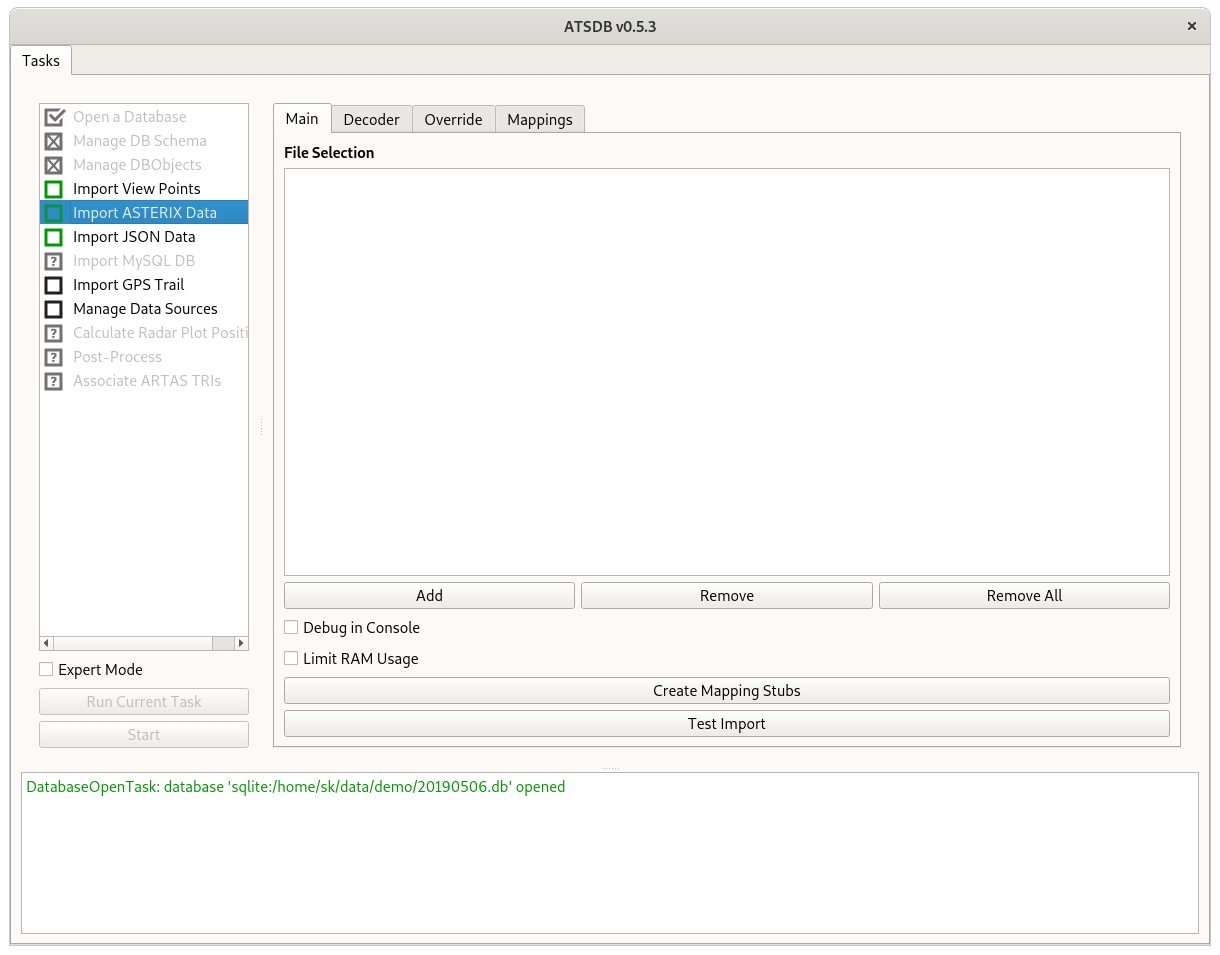
\includegraphics[width=10cm]{../screenshots/asterix_import_data.png}
  \caption{Import ASTERIX Data task}
\end{figure}

In the 'File Selection' list, a list of available ASTERIX data files is given. Entries can be added using the 'Add' button or removed using the 'Remove' buttons. Please add and select the file to be imported.\\

In the 'ASTERIX Configuration' widget the framing, which categories are to be encoded and the currently acitive editions can be set.

Further below, the list of existing JSON object parsers is shown. Each parser parses JSON data and maps to a specific DBO. 

To inspect or edit a JSON object parser, click on it in the list. This step is not required for parsing, but it does give information which ASTERIX content is skipped and which is parsed, and to DBObject variable it is written. \\\\

Using the 'Debug in Console' checkbox, additional debugging information is output to the console, and the ASTERIX decoding is switched to single-threading for easier investigation.

Using the 'Test Import' button, the import function can be tested without inserting the data into the database, the 'Import' imports the selected file with the given options. \\

During import a status indication will be shown:

\begin{figure}[H]
  \center
    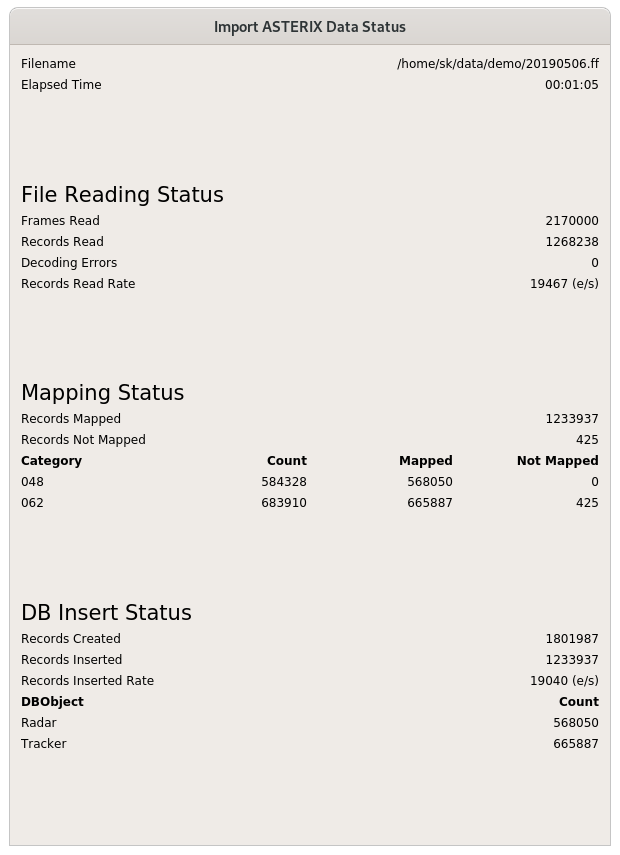
\includegraphics[width=12cm]{../screenshots/asterix_import_status.png}
  \caption{Import ASTERIX data task status}
\end{figure}

If an decoding error occurs, a brief message box is shown, after which the application has to be closed. Please make sure that the correct framing and edition versions are selected, or contact the author for support if this does not resolve the issue. \\

After import, a confirmation will be shown:

\begin{figure}[H]
  \center
    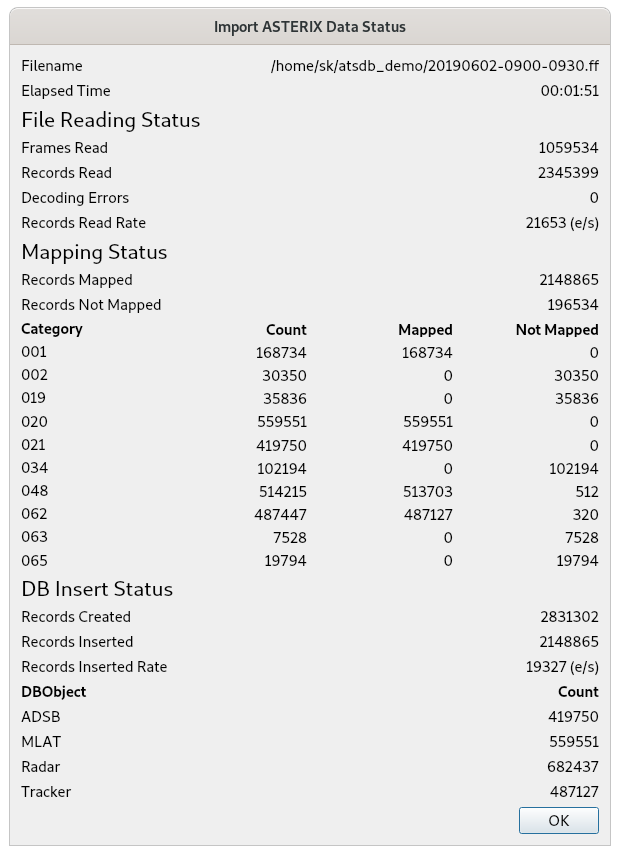
\includegraphics[width=10cm]{../screenshots/asterix_import_done.png}
  \caption{Import ASTERIX data task done}
\end{figure}

Importing performance strongly depends on CPU performance (multi-threading very beneficial), but a import of 2.8 million target reports takes about 2 minutes on the author's hardware. \\


\includegraphics[width=0.5cm]{../../data/icons/hint.png} Please also note the currently not all data fields (as shown in the JSON object parsers) are imported.\\

The (truncated) timestamps of CAT001 are calculated in a simple algorithm based on the CAT002 messages from the same sensor, so their timestamp data is slightly unreliable, but exact enough for e.g. time window filtering. \\\\


\includegraphics[width=0.5cm]{../../data/icons/hint.png} After the import it is recommended to re-start the application, since currently a memory leak during import exists. While this does not affect the import process, usage of the application directly after the import process will be slower than usual. A re-start of the application resolves this issue. This will be fixed in the next version. \\ 
